% Anexo V — Planimetría de detalles estructurales. Origen: láminas 3.1 y 3.2 (PDF vectorial, 2026-11-19).
\chapter{Planimetría de detalles estructurales}
\label{anx:planimetria-estructural}

Las \cref{fig:lamina-3-1,fig:lamina-3-2} presentan los detalles estructurales de la plataforma de soporte de los estanques de almacenamiento.

\begin{figure}[p]
  \centering
  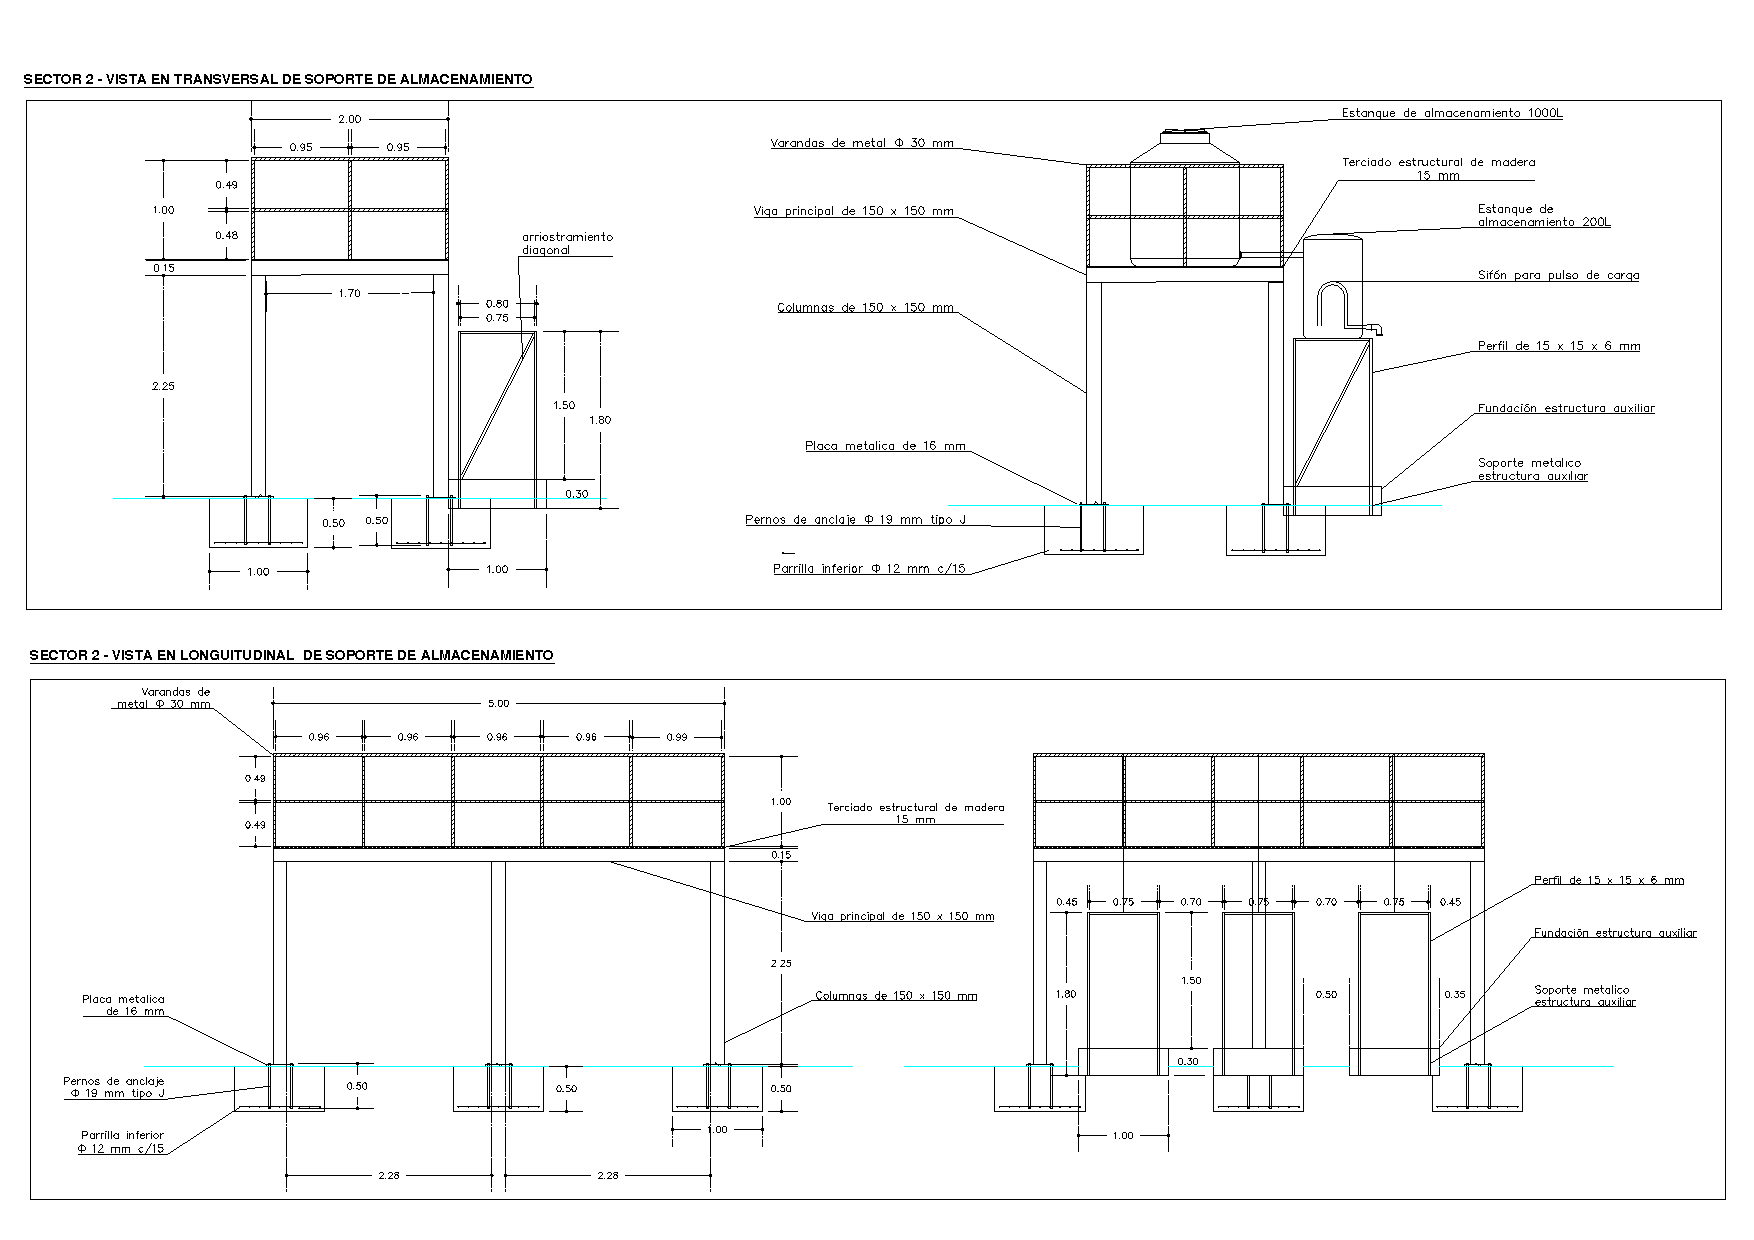
\includegraphics[angle=90, height=0.82\textheight, width=\textwidth, keepaspectratio]{planos/3_1_detalle-estructural-plataforma.pdf}
  \caption{Lámina 3.1: vistas transversal y longitudinal de la estructura de soporte de almacenamiento. Fuente: elaboración propia.}
  \label{fig:lamina-3-1}
\end{figure}

\begin{figure}[p]
  \centering
  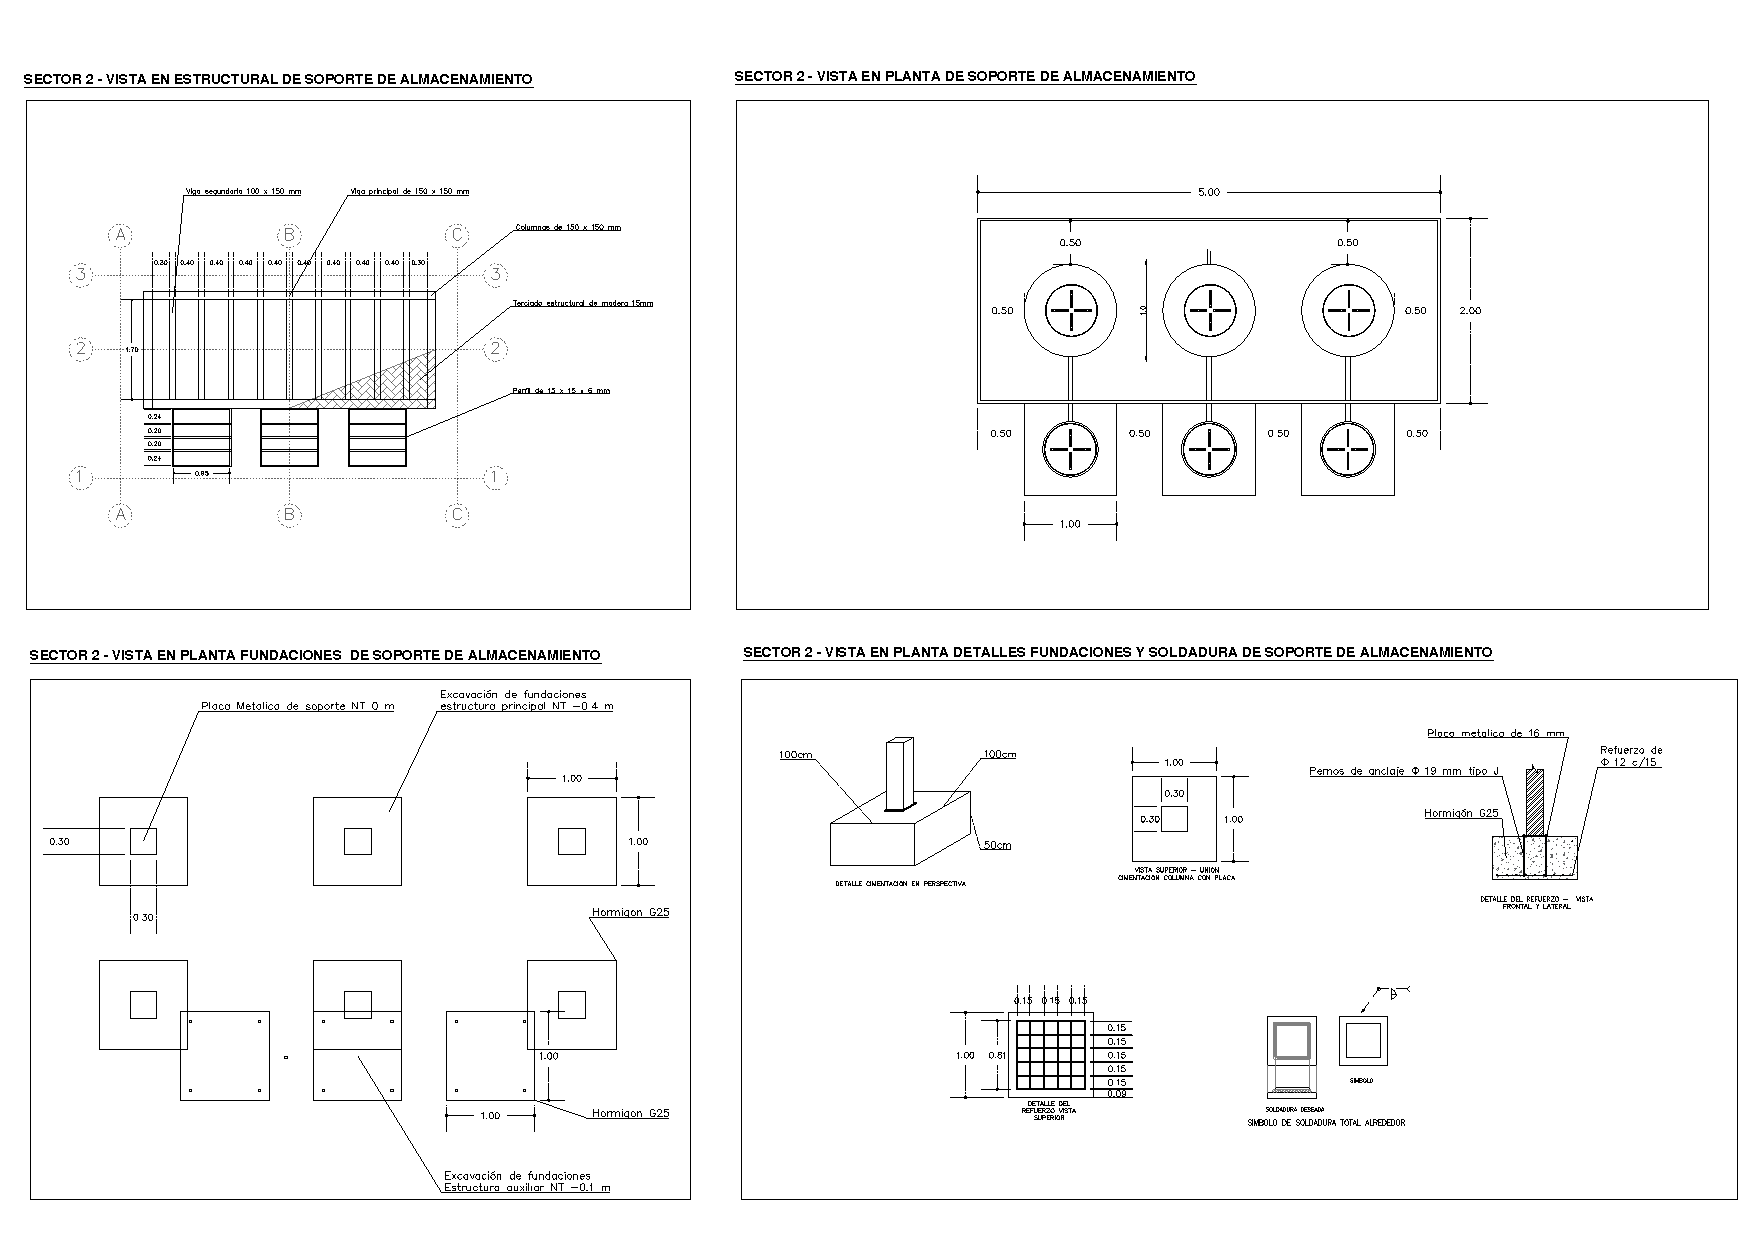
\includegraphics[angle=90, height=0.82\textheight, width=\textwidth, keepaspectratio]{planos/3_2_detalle-estructural-plataforma.pdf}
  \caption{Lámina 3.2: planta estructural, planta de fundaciones y detalles de fundaciones y soldadura. Fuente: elaboración propia.}
  \label{fig:lamina-3-2}
\end{figure}

\revisar{En la lámina 2.4 tengo que corregir la cota de los estanques (\qty{124.27}{\meter} en vez de \qty{125.27}{\meter}), y verificar la profundidad de las fundaciones de la estructura auxiliar (NT $-$\qty{0.1}{\meter} en la lámina 3.2 frente a unos \qty{0.50}{\meter} en la 3.1).}
